%\documentclass[a4paper,doc]{apa6}
\documentclass[a4paper]{article}
% \graphicspath{{/figures/}{./../figures/}}

\usepackage[english]{babel}
\usepackage[utf8x]{inputenc}
\usepackage[colorlinks=true, urlcolor=blue, citecolor=blue, linkcolor=blue]{hyperref}

\usepackage{apacite}
\usepackage{authblk}  % for authors
\usepackage{xcolor}
\definecolor{mypink}{RGB}{255, 230, 255}

\usepackage{nicefrac}
\usepackage{amsmath}
\usepackage{graphicx}
\usepackage{chngcntr} % appendix references
\usepackage[colorinlistoftodos,prependcaption]{todonotes}
\usepackage{pgfplotstable}
\pgfplotstableset{
	fixed zerofill,
	precision=3,
	col sep = comma,
	search path={../tables/}
}
\pgfkeys{/pgf/number format/precision=2, /pgf/number format/fixed}%

\newcommand{\getValue}[3]{%
	\pgfplotstablegetelem{#1}{#2}\of{#3}%
	\pgfmathprintnumber{\pgfplotsretval}%
}
\newcommand{\setValue}[4]{%
	\pgfplotstablegetelem{#1}{#2}\of{#3}%
	\pgfmathprintnumberto{\pgfplotsretval}{#4}%
}


\newcommand{\getCI}[2]{[\getValue{#1}{Lower}{#2}, \getValue{#1}{Upper}{#2}]}

\usepackage{titlesec}

\titlespacing\section{0pt}{8pt plus 4pt minus 2pt}{4pt plus 2pt minus 2pt}
\titlespacing\subsection{0pt}{8pt plus 4pt minus 2pt}{0pt plus 2pt minus 2pt}
\titlespacing\subsubsection{0pt}{8pt plus 4pt minus 2pt}{0pt plus 2pt minus 2pt}

\usepackage{tikz}
\usepackage{tikzscale} % check if used!

\usepackage[most]{tcolorbox}

\newtcolorbox[auto counter]{NewBox2}[2][]{
	colframe=black,colback=white,
	enhanced,
%	breakable,
	title={Box \thetcbcounter: #2},
	colbacktitle=white,
	coltitle = black,
	detach title,
	before upper={\tcbtitle\quad},
	#1
}
%\getValue{0}{ph0}{\reanalysis}

\newcommand{\EJ}[1]{\todo[inline, color=green]{  #1 }}
\newcommand{\Q}[1]{\todo[inline, color=yellow]{  #1 }}
\newcommand{\jv}[2]{{\color{red}\st{#1}}{\color{blue}\bf{#2}}}
\newcommand{\DON}[1]{\todo[inline, color=white]{Don: #1}}
\newcommand{\DONside}[1]{\todo[color=white]{#1}}
%\newcommand{\DONTODO}[1]{{\color{red}{#1}} \addcontentsline{tdo}{todo}{#1}}
\newcommand{\J}[1]{\todo[inline, color=mypink]{#1}}

\graphicspath{{../figures/}}
\newcommand{\hypo}[1]{\ensuremath{\mathcal{H}_{#1}}}
\newcommand{\model}{\mathcal{M}}
\newcommand{\data}{\mathrm{data}}%\mathcal{D}}
\newcommand{\midd}{\ensuremath{\,|\,}}
\newcommand{\cohend}{\ensuremath{d}}
\newcommand{\prob}{\mathrm{Pr}}

\newcommand{\osflink}{\url{https://osf.io/uq8st/}}

\newcommand{\CamererReplication}{\url{https://mfr.osf.io/render?url=https://osf.io/fg4d3/?action=download\%26mode=render}}
\newcommand{\manyLabsLink}{\url{https://mfr.osf.io/render?url=https://osf.io/xufw4/?action=download\%26mode=render}}


\title{A Cautionary Note on Estimating Effect Sizes}
%\shorttitle{Estimating Effect Size} 
\renewcommand{\thefootnote}{\fnsymbol{footnote}}
\author[1]{Don van den Bergh%
	\thanks{Correspondence concerning this article should be addressed to: Don van den Bergh, University of Amsterdam, Department of Psychological Methods, Nieuwe Achtergracht 129B, 1018VZ Amsterdam, The Netherlands. E-Mail should be sent to: donvdbergh@hotmail.com.
}}
\author[1]{Julia M. Haaf}
\author[1,2]{Alexander Ly}
\author[3]{\authorcr Jeffrey N. Rouder} % putt Jeff on a newline to avoid a newline after his first name
\author[1]{Eric-Jan Wagenmakers}
\affil[1]{University of Amsterdam}
\affil[2]{Centrum Wiskunde \& Informatica}
\affil[3]{University of California Irvine}
\date{}
%\affiliation{~}
\renewcommand*{\thefootnote}{\arabic{footnote}}
%
%\threeauthors{Don van den Bergh and Julia M. Haaf and Alexander Ly and Eric-Jan Wagenmakers}{Alexander Ly}{Jeffrey N. Rouder}
%\threeaffiliations{University of Amsterdam}{Centrum Wiskunde \& Informatica}{University of California Irvine}
%\authornote{Correspondence concerning this article should be addressed to: Don van den Bergh, University of Amsterdam, Department of Psychological Methods, Nieuwe Achtergracht 129B, 1018VZ Amsterdam, The Netherlands. E-Mail should be sent to: donvdbergh@hotmail.com.}

\pgfplotstableread{effectSizeExample.csv}\tbEffectSizeExample
\pgfplotstableread{posteriorProbH0.csv}\reanalysis

\begin{document}

%\listoftodos
%\newpage

\maketitle

\begin{abstract}
	An increasingly popular approach to statistics is to focus on estimation and to forgo hypothesis testing altogether. Through an example, we show that estimates and confidence of effect sizes are overestimated the null is ignored, and when it is a plausible description of the data. We illustrate how this overestimation can be avoided by incorporating the plausibility of the null into the estimation process.
\end{abstract}

Consider the following scenario: Your colleague has just conducted an experiment for a Registered Report. The analysis yields $p<0.05$ and your colleague believes that the null hypothesis can be rejected. In line with recommendations both old \cite<e.g., >{Grant1962, Loftus1996} and new \cite<e.g., >{harrington2019new, Cumming2014} you convince your colleague that it is better to replace the $p$-value with an estimate of the effect size and a 95\% confidence interval \cite<but see>{MoreyEtAl2016CI}. You also manage to convince your colleague to plot the data. Instead of simply reporting $p<0.05$, the statistical analysis in the report is now more informative. The result is shown in Figure~\ref{fig:descriptivesPlot}. In the text of the paper, the result is summarized as Cohen's $\cohend = \getValue{0}{Estimate}{\tbEffectSizeExample}$, CI $= \getCI{0}{\tbEffectSizeExample}$, in line with guidelines for reporting statistics (e.g., the guidelines of the Psychonomic Society\footnote{\protect\url{https://www.springer.com/psychology?SGWID=0-10126-6-1390050-0}}, or those of Psychological Science\footnote{\url{https://www.psychologicalscience.org/publications/psychological\_science/ps-submissions\#STAT}}).
\begin{figure}[!ht]
	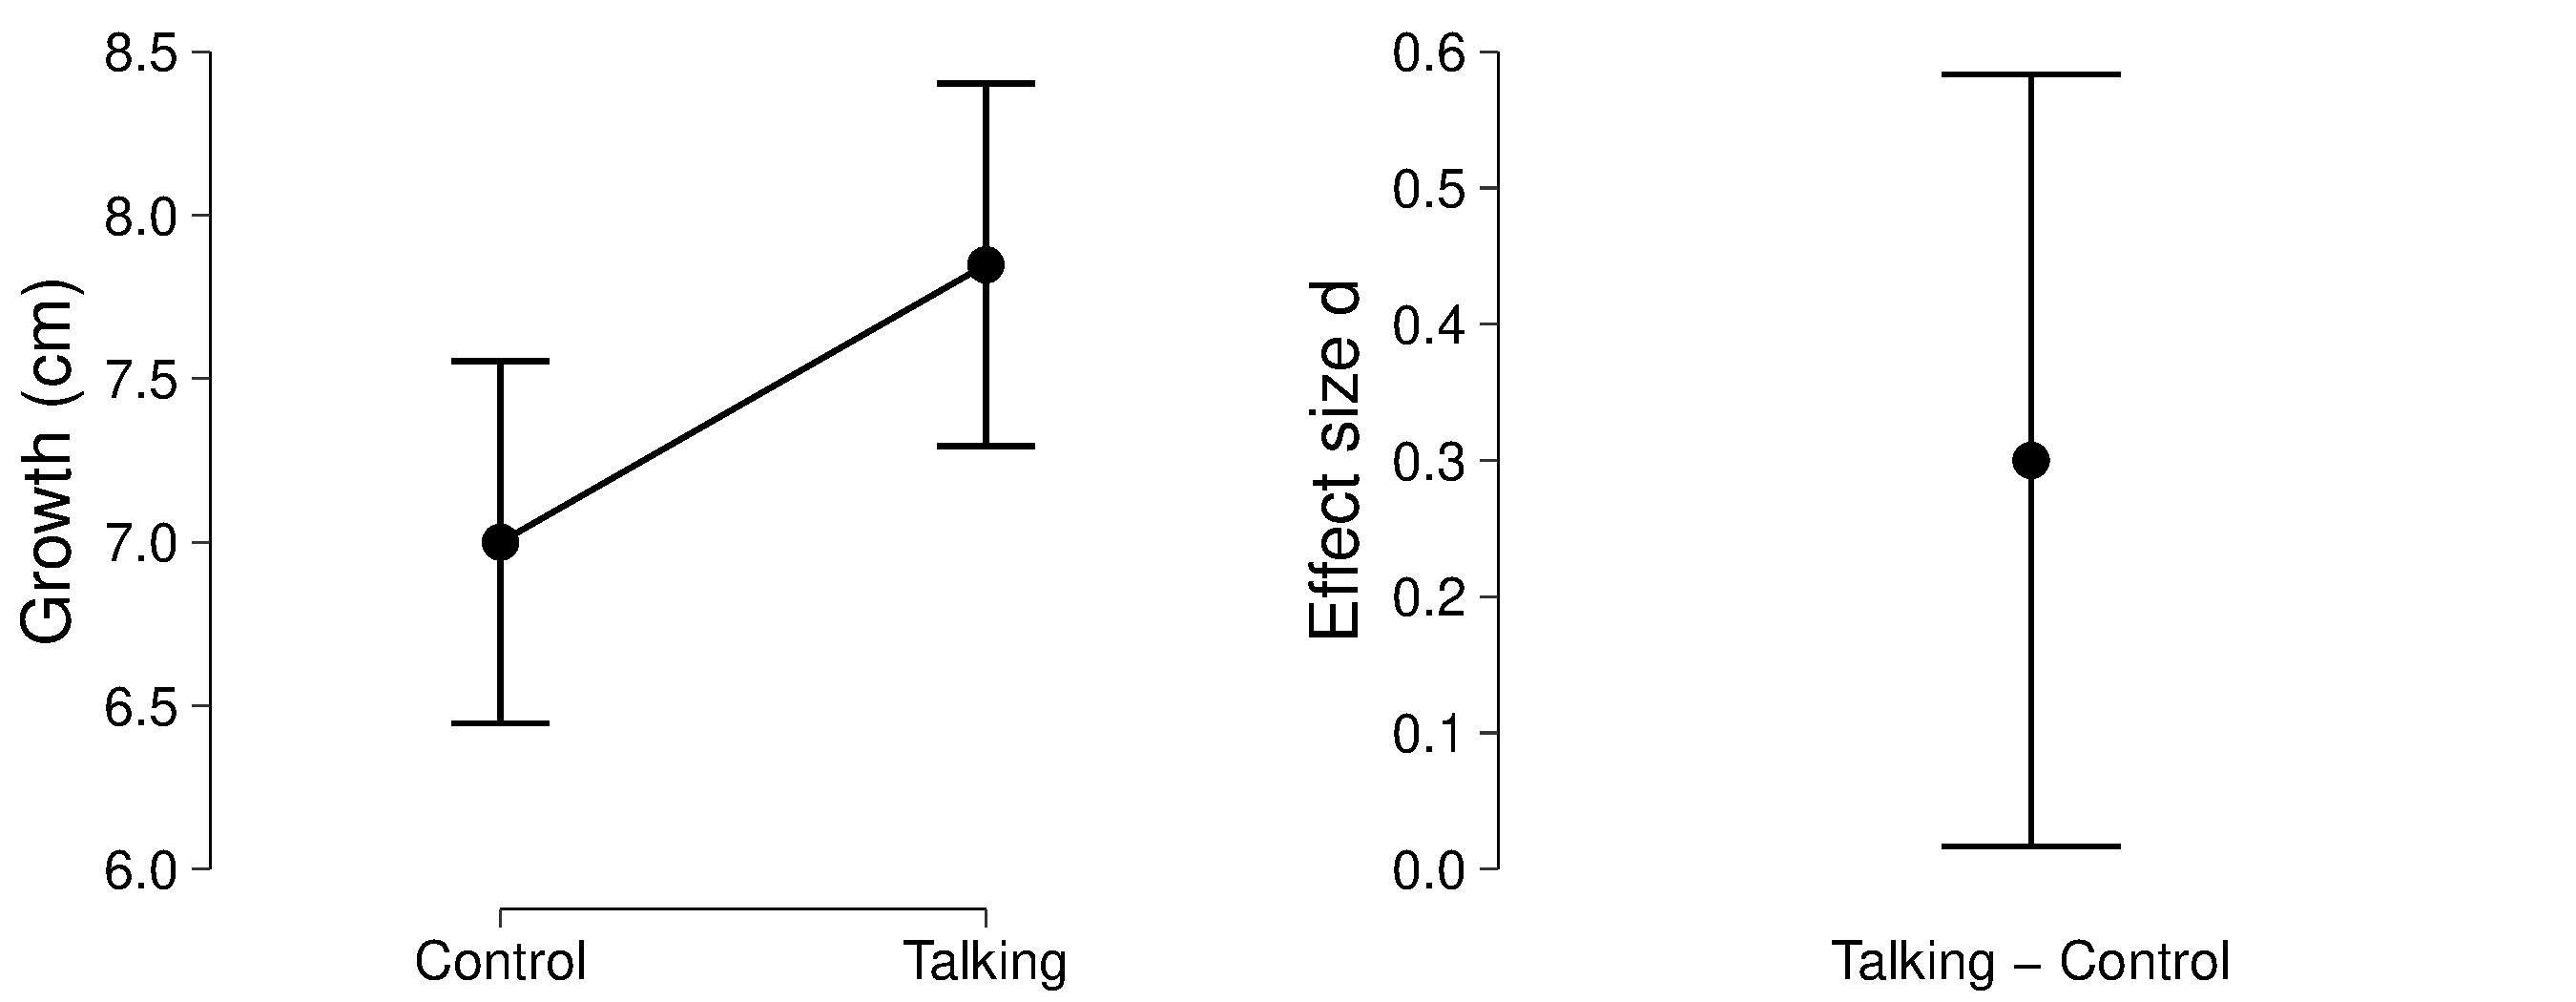
\includegraphics[width=\textwidth]{descriptivesPlot.pdf}
	\caption{The left panel shows a descriptives plot with the mean and 95\% confidence interval of the simulated plant growth. The right panel shows an estimate of the effect size, Cohen's \cohend, and a 95\% confidence interval.}
	\label{fig:descriptivesPlot}
\end{figure}
Given the results shown in Figure~\ref{fig:descriptivesPlot}, what is a reasonable point estimate of the effect size? A straightforward answer is ``\getValue{0}{Estimate}{\tbEffectSizeExample}'' which makes intuitive sense from an estimation perspective. However, your colleague now tells you about the nature of the experiment: plants grow faster when you talk to them.\footnote{Specifically, imagine your colleague took 100 plants and measured their growth three times during two weeks. The first week 50 plants were randomly selected and spoken to while the other served as control. The next week, the roles reversed and the previously spoken to plants served as controls while the control plants were now talked to. The quantity of interest is the difference in growth between the weeks. This example is inspired by \protect\citeA{BergerDelampady1987}.} Suddenly, a population effect size of ``0'' also appears plausible. Any observed difference may merely be due to the individual differences between the plants.\footnote{Unless you talk out loud, with consumption, and the plant is near.}

\section*{When are Effect Sizes Overestimated?}
Standard point estimates and confidence intervals are based solely on the alternative hypothesis and therefore tend to overestimate effect sizes. This overestimation is caused by the strong assumption that the null hypothesis is irrelevant. However, the null can have high plausibility after seeing the data. This happens if the alternative is a-priori unlikely (e.g., for a null hypothesis like ``Talking to plants does not affect their growth.''), or when the data are so uninformative that after seeing the data there is substantial uncertainty about which model is best. If the null hypothesis still has a high plausibility after seeing the data, it is obvious that it cannot be ignored, but that is exactly what is done when estimates are only based on the alternative hypothesis. As a result, the estimates are overconfident and, because the null hypothesis would shrink the estimates towards zero, overestimated.

\section*{A Spike-and-Slab Perspective}
Here, we illustrate the overestimation and a remedy against it by reanalyzing the fictitious data from Figure~\ref{fig:descriptivesPlot}.\footnote{R code for the analysis is available at \osflink{}.} We consider the spike-and-slab model \cite{RouderEtAl2018PBR, clyde1996prediction, mitchell1988bayesian}, which consists of two components. The first component corresponds to the position that talking to plants does not make them grow faster or slower ($\cohend = 0$). The second component corresponds to the position that  speaking to plants does influence their growth ($\cohend \neq 0$). A-priori both components are equally likely; the prior probability each component is \nicefrac{1}{2}. Here we view the spike-and-slab as a single model, although it can also be viewed as a form of Bayesian model averaging (see Box~\ref{box:box1} for more details). Typically, an estimate of the effect size is solely based on the second component, which yields a point estimate and an uncertainty interval (for frequentists, $\cohend = \getValue{0}{Estimate}{\tbEffectSizeExample}$, 95\%  CI: \getCI{0}{\tbEffectSizeExample}; for Bayesians $\cohend = \getValue{1}{mean}{\reanalysis}$, 95\% CRI: \getCI{1}{\reanalysis}). The spike-and-slab model, however, also considers the possibility that an effect can be exactly zero and thus the estimate is an average of the two components and thus shrunken towards zero.\footnote{For the spike-and-slab model, the posterior distribution is constructed in the following manner: $p(\delta\midd\data) = 1\{\delta = 0\}\prob(\model_0\midd\data) + p(\delta\midd\data,\model_1)\prob(\model_1\midd\data)$. Here, $1\{\delta = 0\}$ is the Dirac delta function which represents the spike under the null, $\prob$ denotes probability of a model, and $p$ denotes density related to the magnitude of the effect.} Figure 2 contrasts inference based on one component with inference based on both components by showing their 95\% credible intervals and posterior means.
% these cannot be generated inside the caption
\setValue{0}{ph1}{\reanalysis}{\phAlt}%
\setValue{0}{mode}{\reanalysis}{\modeAlt}%
\begin{figure}[!ht]
	\centering
	\begin{tikzpicture}
		\node[anchor=south west,inner sep=0] (image) at (0,0) {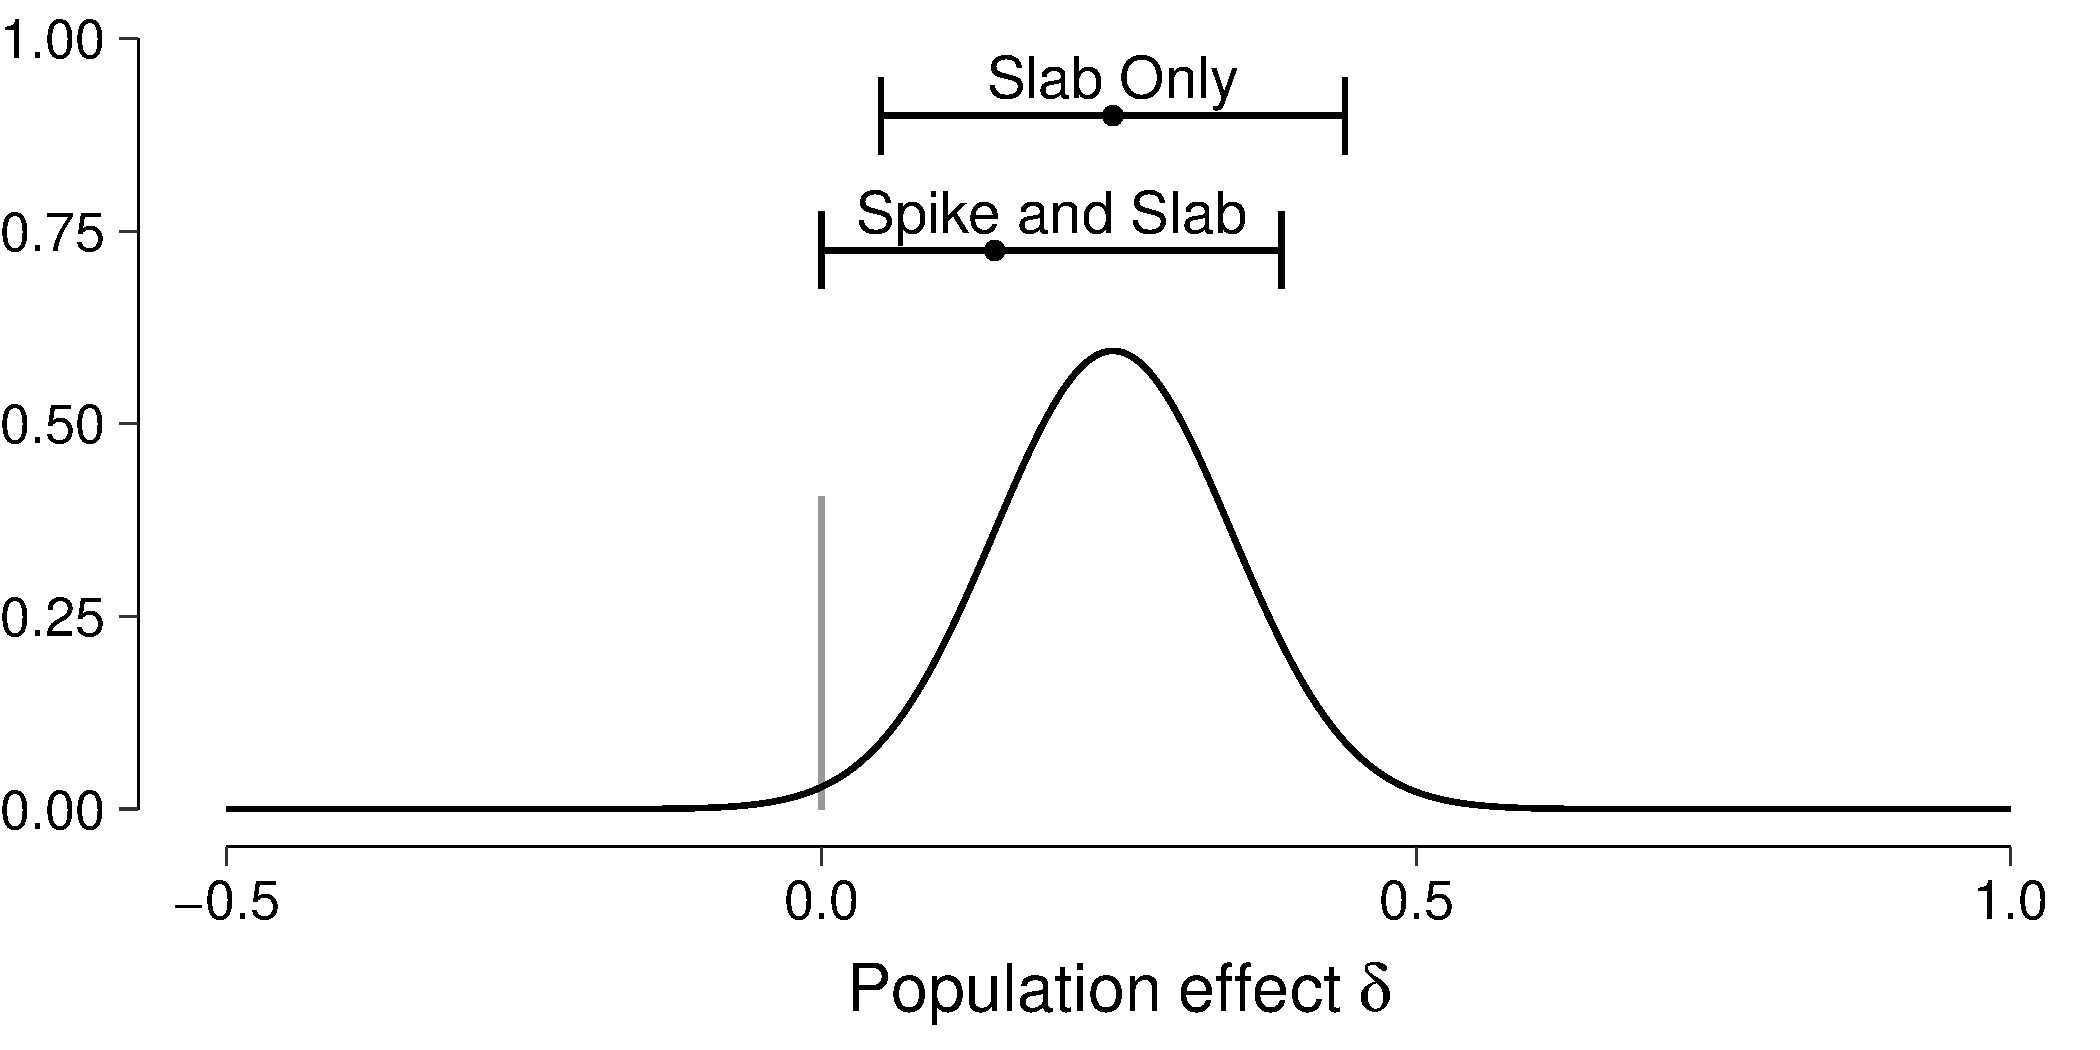
\includegraphics[width=0.9\textwidth]{spikeAndSlabPosteriorRescaledPosteriorMode.pdf}};
		\begin{scope}[x={(image.south east)},y={(image.north west)}]
		\node[anchor=base,inner sep=0pt, outer sep=0pt] at (0.28,0.61) {$p(\hypo{0}\mid\data) = \getValue{0}{ph0}{\reanalysis}$};
		\end{scope}
	\end{tikzpicture}
	\caption{
		Visualization of the results from the spike-and-slab model. The black line represents the posterior distribution of effect size given the slab (i.e., the effect is non-zero). The posterior is scaled so that its mode ($\delta = \modeAlt$) equals the posterior probability of the alternative model (i.e., $p(\hypo{1}\mid\data) = \phAlt$). The grey line represents the posterior probability of the spike (i.e., the effect is exactly 0). The error bars and dots above the density show 95\% credible intervals and the posterior mean for a posterior based on only the slab and for a posterior based on the spike-and slab.}
	\label{fig:modelAveragedPosterior}
\end{figure}
The posterior mean and central 95\% credible interval of the spike-and-slab model are shrunken towards 0 compared to the results based on only the slab (i.e., \getValue{0}{mean}{\reanalysis} (95\% CRI: \getCI{0}{\reanalysis}) vs. \getValue{1}{mean}{\reanalysis} (95\% CRI: \getCI{1}{\reanalysis})). This shrinkage is caused by the non-negligible probability that the effect is absent. Although 0 appears to be included in the credible interval, this cannot be interpreted directly as evidence against an effect. Instead, the spike-and-slab posterior simultaneously contains evidence for the presence of the effect and an estimate of the magnitude of the effect across the two components. Note that as the posterior probability of the null decreases, the spike-and-slab results approach those of the alternative model.

\section*{Discussion}
We argue that estimates of effect sizes based only on the alternative hypothesis tend to be overconfident, in particular when a null hypothesis may also describe the data well. Consequently, point estimates and confidence intervals based solely on the alternative overestimate effect sizes. A solution for this overestimation is the spike-and-slab model which explicitly considers the possibility that an effect is exactly 0 \cite<as is also advocated for by>{KiersTendeiro2019, RouderEtAl2018PBR}. Although this idea is not new, the influence of the null is still too often ignored in practice.

%\subsubsection*{Extending the Null to a Perinull}
\subsubsection*{All Null Hypotheses are False}
The spike-and-slab approach may contrast with the popular estimation mindset, where it is argued that statistical significance should be abandoned in favor of estimation \cite{McShane2019abandon, valentine2015life, Cumming2014}. An argument to forgo hypothesis testing is that all null hypotheses are false \cite{Cohen1990, Meehl1978} and therefore there is no need to consider a component that states that an effect is exactly zero. However, a statistical argument to consider point nulls is that they accurately approximate intervals near zero \cite{BergerDelampady1987}. Thus, it is irrelevant whether null hypotheses are exactly true. Furthermore, several large-scale replications studies have demonstrated that a near-zero effect size is reasonable in practice, i.e., the null can be a plausible description of the data \cite<e.g., see the meta-analyses conducted by>{CamererEtAl2018, KleinEtAl2018ML2, NosekLakens2014}. Moreover, the spike need not always represent a null of exactly zero; it could also represent a perinull ---a region near zero that represents ``practically irrelevant'' effect sizes. Typically, the perinull spike is a distribution centered around zero with a small variance. Key is that the argument remains unchanged. Since the perinull has most of its mass near zero, estimates will still be shrunk towards zero. Thus the null is not ignored and overestimation is avoided. For a comparison of null and perinull spikes, see \citeA{malsiner2018comparing}.

\subsubsection*{When (not) to Consider the Spike}
The main reason to ignore the spike is when overestimation is implausible. This happens in two scenarios: First, when prior research indicates that the prior probability of the spike is negligible, the spike can safely be ignored. For example, if we estimate the popularity of two politicians, a spike that represents that the two politicians are equally popular is so implausible that it can be ignored. Second, when the data provide overwhelming evidence that an effect is non-zero, the results from a spike-and-slab model become virtually identical to those of a slab only model and thus the spike can be ignored. For instance, when the data show that one politician is 10 times as popular as another, the posterior probability of the spike that states the politicians are equally popular is nearly zero. A practical recommendation is to ignore the spike whenever the sample size is larger than 50 and the point estimate (posterior mean or maximum likelihood estimate) is more than three standard deviations away from the spike (\citeNP[p. 193--194]{Jeffreys1939}; \citeNP[p. 75]{Jeffreys1980}). Yet, the spike does not hurt in either of these scenarios.

\subsubsection*{Conclusion}
In sum, we argue that descriptions of effect sizes based on only the alternative hypothesis are overconfident and as a consequence overestimate effect sizes. A remedy for this overestimation is the spike-and-slab model which explicitly accounts for the possibility of the null of no effect. Although this idea is not new, it remains underutilized in practice, and we hope this paper brings more attention to the spike-and-slab approach.

\bibliographystyle{apacite}
\bibliography{referenties, referenties.bib}

\begin{NewBox2}[label=box:box1]{The Spike-and-Slab Distribution as Bayesian Model Averaging}{}%
	\vspace{6pt}\hrule\vspace{6pt}
	The spike-and-slab distribution can be viewed as a single model that consists of two components: the slab, which assumes that the effect is non-zero, and the spike, which assumes the effect is exactly zero. However, the spike-and-slab distribution can also be seen as a form of Bayesian model averaging. From that perspective, the spike and the slab are two individual models. The slab represents the unconstrained model that freely estimates effect size, and the spike represents the constrained model where the effect size is fixed to zero. Next, the results for each model are weighted by the posterior model probabilities and averaged, so that inference can be made using results from both models simultaneously. Such averaging over models provides the best predictive performance (\citeNP[p. 640--641]{ZellnerVandaele1975}, as described in \citeNP[p. 600--601]{ZellnerSiow1980}; \citeNP[p. 57]{Haldane1932}; \citeNP{IversonEtAl2010}; \citeNP{RouderEtAl2018PBR}), and conceptually similar ideas date back much further (\citeNP[p. 387]{WrinchJeffreys1921}; \citeNP{Jevons18741913}). Note that these two perspectives ---a two-component model or averaging of two models--- differ in semantics but are mathematically equivalent.
\end{NewBox2}

\end{document}